\documentclass[border=10pt]{standalone}
\usepackage[svgnames]{xcolor}
\usepackage{amsmath}
\usepackage{pgfplots}
\pgfplotsset{compat=newest}
\usepackage[sfdefault]{FiraSans}
\usepackage{FiraMono}
\renewcommand*\familydefault{\sfdefault}
\begin{document}
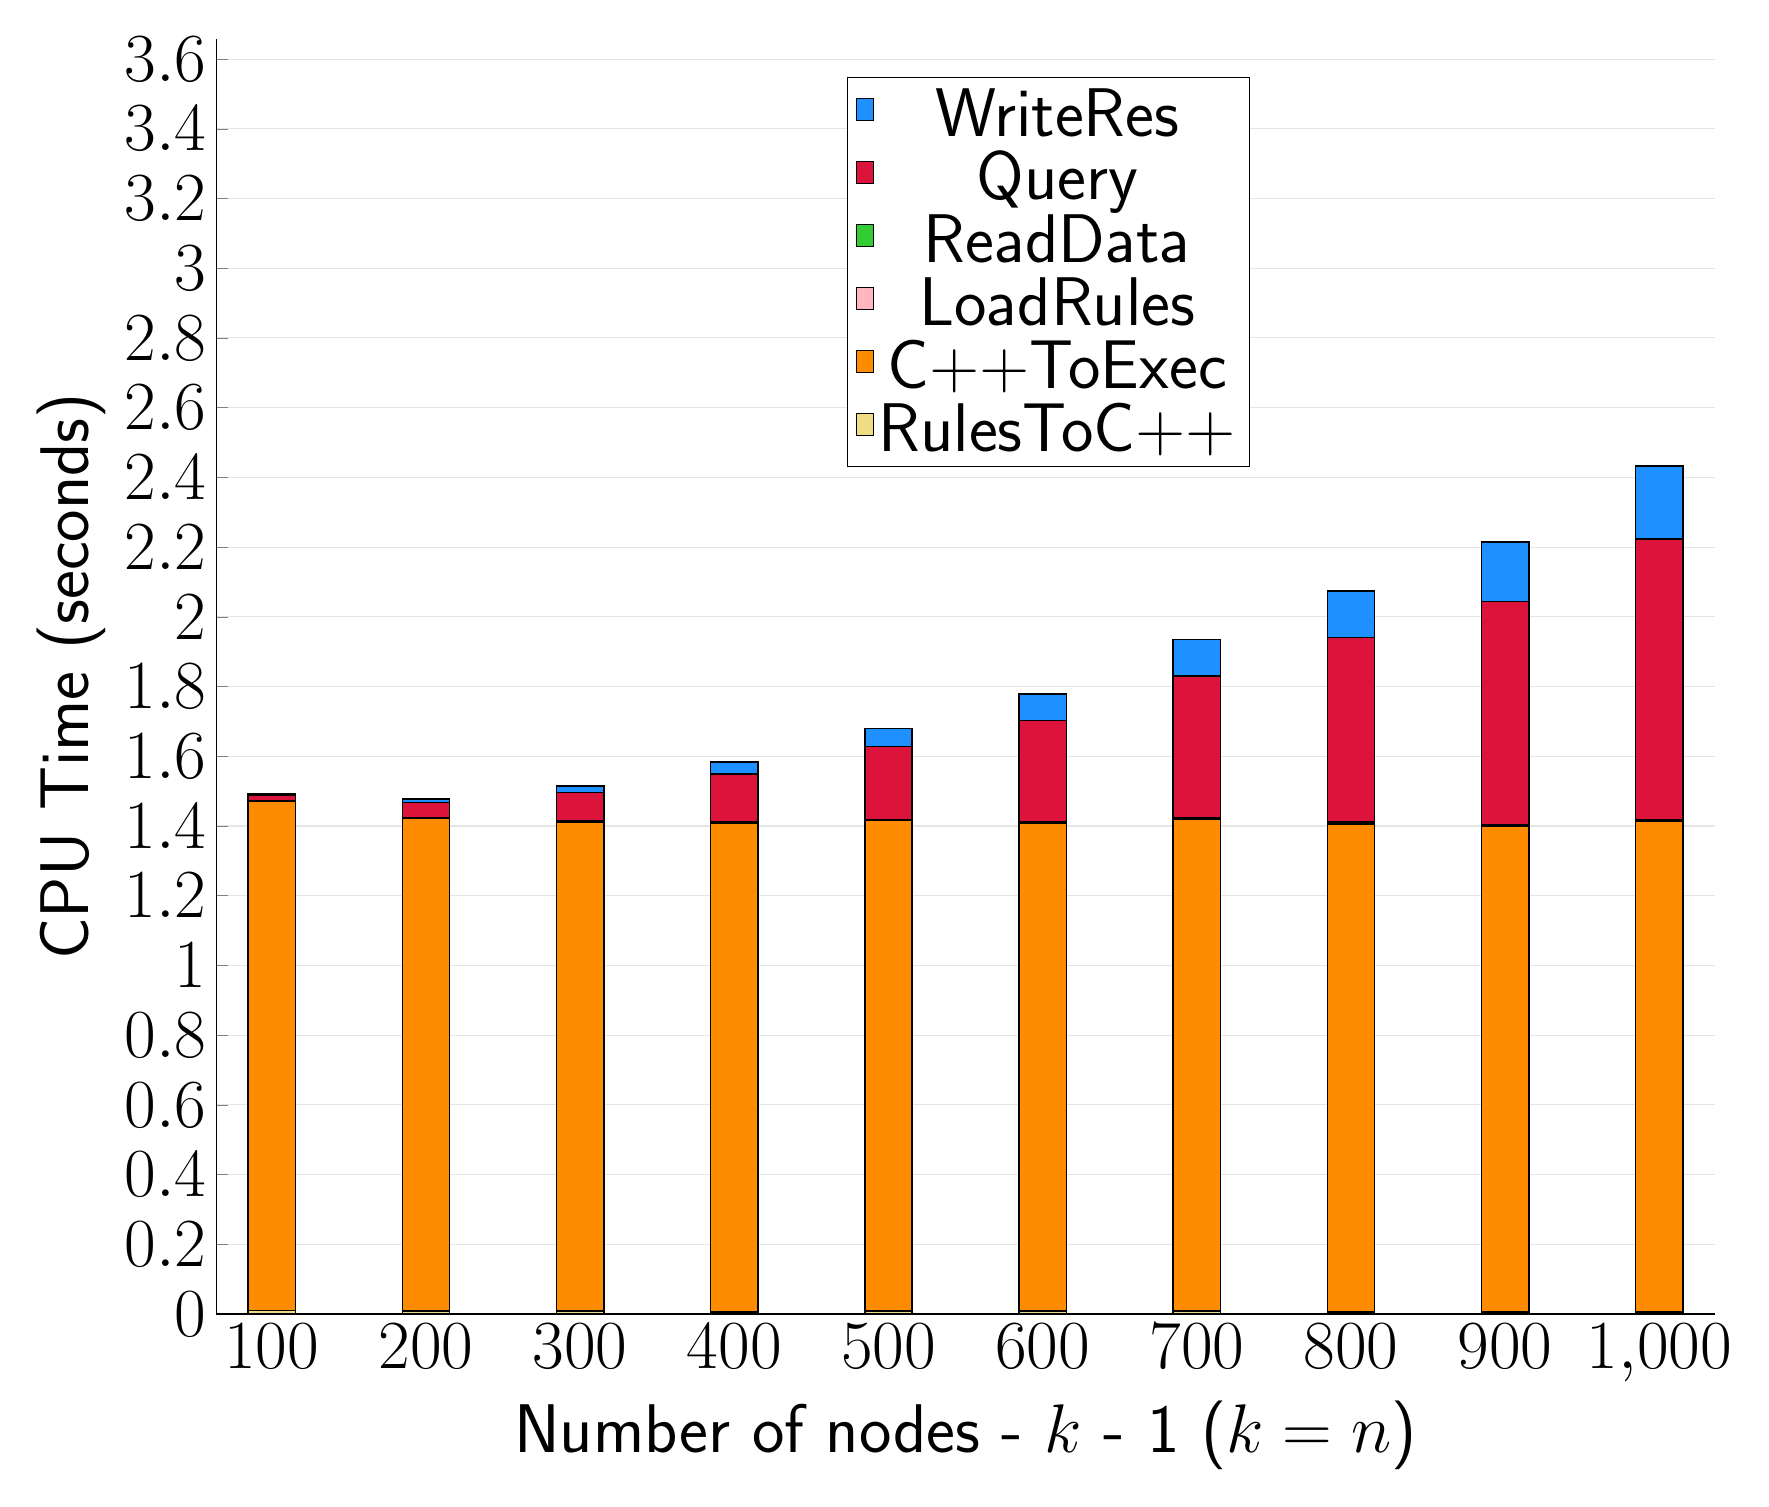
\begin{tikzpicture}
\begin{axis}[
   ybar stacked,
   width=1.7\textwidth,
   bar width=0.6cm,
   ymajorgrids, tick align=inside,
   major grid style={draw=gray!20},
   xtick=data,
   ymin=0, ymax=3.658792,
   axis x line*=bottom,
   axis y line*=left,
   enlarge x limits=0.04,
   legend style={
       at={(0.69, 0.97)},
       anchor=north east,
       legend columns=1,
       font=\Huge,
   },
   ylabel={CPU Time (seconds)},
   xlabel={Number of nodes - $k$ - 1 ($k=n$)},
   label style={font=\Huge},
   tick label style={font=\Huge},
]
\addlegendimage{fill=DodgerBlue, draw=black, line width=0.2pt}
\addlegendentry{WriteRes}
\addlegendimage{fill=Crimson, draw=black, line width=0.2pt}
\addlegendentry{Query}
\addlegendimage{fill=LimeGreen, draw=black, line width=0.2pt}
\addlegendentry{ReadData}
\addlegendimage{fill=LightPink, draw=black, line width=0.2pt}
\addlegendentry{LoadRules}
\addlegendimage{fill=DarkOrange, draw=black, line width=0.2pt}
\addlegendentry{C++ToExec}
\addlegendimage{fill=LightGoldenrod, draw=black, line width=0.2pt}
\addlegendentry{RulesToC++}
\addplot +[fill=LightGoldenrod, draw=black, line width=0.55pt] coordinates {
(100, 0.009999999999999997)
(200, 0.008000000000000002)
(300, 0.007999999999999997)
(400, 0.005999999999999997)
(500, 0.007999999999999997)
(600, 0.007999999999999997)
(700, 0.007999999999999997)
(800, 0.005999999999999997)
(900, 0.005999999999999997)
(1000, 0.005999999999999997)
};
\addplot +[fill=DarkOrange, draw=black, line width=0.55pt] coordinates {
(100, 1.4620000000000002)
(200, 1.4140000000000001)
(300, 1.4040000000000004)
(400, 1.4020000000000004)
(500, 1.4080000000000001)
(600, 1.4000000000000001)
(700, 1.4120000000000001)
(800, 1.4000000000000004)
(900, 1.394)
(1000, 1.4080000000000001)
};
\addplot +[fill=LightPink, draw=black, line width=0.55pt] coordinates {
(100, 0.00015319999999999998)
(200, 0.00016059999999999997)
(300, 0.00011640000000000001)
(400, 0.0001562)
(500, 0.00011520000000000001)
(600, 0.0001488)
(700, 0.00016219999999999999)
(800, 0.0001636)
(900, 0.00010339999999999999)
(1000, 0.000108)
};
\addplot +[fill=LimeGreen, draw=black, line width=0.55pt] coordinates {
(100, 0.0010078)
(200, 0.0014678)
(300, 0.0019124000000000003)
(400, 0.0028398)
(500, 0.0029477999999999996)
(600, 0.0031157999999999997)
(700, 0.0043156)
(800, 0.0046657999999999995)
(900, 0.0046616)
(1000, 0.0050688)
};
\addplot +[fill=Crimson, draw=black, line width=0.55pt] coordinates {
(100, 0.0161912)
(200, 0.0434458)
(300, 0.0819602)
(400, 0.138382)
(500, 0.2092698)
(600, 0.29195840000000006)
(700, 0.40596639999999995)
(800, 0.5293294)
(900, 0.6390182)
(1000, 0.8041834000000001)
};
\addplot +[fill=DodgerBlue, draw=black, line width=0.55pt] coordinates {
(100, 0.0043175999999999996)
(200, 0.010116)
(300, 0.0193822)
(400, 0.034049800000000005)
(500, 0.051759200000000005)
(600, 0.07514760000000001)
(700, 0.1038238)
(800, 0.1339656)
(900, 0.1711442)
(1000, 0.20984179999999997)
};
\end{axis}
\end{tikzpicture}

\end{document}
